% !TEX program = xelatex
% FluxReel — Project Profile Document
% Compile: xelatex -interaction=nonstopmode project_profile.tex
\documentclass[UTF8,fontset=mac,a4paper,11pt]{ctexart}

\usepackage[a4paper,margin=2.4cm,top=2.3cm,bottom=2.4cm]{geometry}
\usepackage{booktabs}
\usepackage{graphicx}
\usepackage{xcolor}
\usepackage{listings}
\usepackage{fontspec}
\usepackage{hyperref}
\usepackage{titlesec}
\usepackage{enumitem}
\usepackage{tabularx}
\usepackage{fancyhdr}
\usepackage{tikz}

% ── fonts ────────────────────────────────────────────────────────────
\setmonofont{Menlo}[Scale=0.85]   % box-drawing friendly monospace

% ── colors (FluxReel / AMD palette) ──────────────────────────────────
\definecolor{amdred}{HTML}{ED1C24}
\definecolor{accent}{HTML}{1E2637}
\definecolor{codebg}{HTML}{F4F6FA}
\definecolor{dimgray}{HTML}{5B6573}

% ── headings ─────────────────────────────────────────────────────────
\titleformat{\section}
  {\Large\bfseries\color{accent}}{\thesection}{0.7em}{}
\titleformat{\subsection}
  {\large\bfseries\color{accent}}{\thesubsection}{0.7em}{}
\titlespacing{\section}{0pt}{1.1em}{0.5em}
\titlespacing{\subsection}{0pt}{0.9em}{0.35em}

% ── page style ───────────────────────────────────────────────────────
\pagestyle{fancy}
\fancyhf{}
\fancyhead[L]{\small\color{dimgray}FluxReel — Project Profile}
\fancyhead[R]{\small\color{dimgray}AMD AI DevMaster Hackathon · Track 1}
\fancyfoot[C]{\small\thepage}
\renewcommand{\headrulewidth}{0.4pt}

% ── listings ─────────────────────────────────────────────────────────
\lstdefinestyle{pp}{
  basicstyle=\ttfamily\footnotesize,
  backgroundcolor=\color{codebg},
  frame=single,
  rulecolor=\color{black!20},
  columns=fullflexible,
  keepspaces=true,
  xleftmargin=8pt,
  xrightmargin=8pt,
  aboveskip=8pt,
  belowskip=10pt,
}
\lstset{style=pp}

% ── links ────────────────────────────────────────────────────────────
\hypersetup{
  colorlinks=true,
  linkcolor=accent,
  urlcolor=amdred,
  pdftitle={FluxReel — Project Profile Document},
  pdfauthor={Zhiwei Li; Thomas Yang (Aztice)},
}

\setlist{topsep=3pt, itemsep=2pt, parsep=0pt}

% English figure/table captions (ctex defaults to 图/表)
\renewcommand{\figurename}{Figure}
\renewcommand{\tablename}{Table}

\begin{document}

% ═══════════════════════════════════════════════════════════════════════
%  Title page
% ═══════════════════════════════════════════════════════════════════════
\begin{titlepage}
  \centering
  {\color{amdred}\rule{\linewidth}{2.5pt}}\\[2.4em]
  {\Huge\bfseries FluxReel}\\[0.7em]
  {\LARGE AMD GPU-Powered Short-Video Creation Tool}\\[2.2em]
  {\large\bfseries Project Profile Document}\\[0.5em]
  {\large Track 1 --- Multimodal Content Creation Tools}\\[1.0em]
  {\large AMD AI DevMaster Hackathon · 2026-07}\\[3.2em]

  \begin{tabular}{@{}l l l@{}}
    \toprule
    & \textbf{Zhiwei Li} & \textbf{Thomas Yang (Aztice)} \\
    \midrule
    Role
      & Senior AI Full-Stack Engineer
      & HK secondary school student · AI infra engineer \\
    Experience
      & 12 years engineering \& entrepreneurship
      & Multiple years in AI infrastructure \\
    GitHub
      & \texttt{github.com/lzwjava}
      & \texttt{github.com/aztice} \\
    \bottomrule
  \end{tabular}

  \vfill
  {\small\color{dimgray}
   One topic · one AMD Radeon GPU · one 15-second video — fully local.}\\[0.6em]
  {\color{amdred}\rule{\linewidth}{2.5pt}}
\end{titlepage}

% ═══════════════════════════════════════════════════════════════════════
\section{Project Background}
% ═══════════════════════════════════════════════════════════════════════

Short video has become the dominant content format across platforms such as
Douyin, WeChat Video Account, and Reels. Yet producing an explainer video
today is a manual, multi-step chore: write a script, source or generate
images, add captions, pick music, and edit everything together --- typically
\textbf{hours of work per video}. Existing automation options are either
cloud APIs that \emph{charge per video} or tools that \emph{upload content
to the cloud}, which is a deal-breaker for privacy-sensitive material.

\textbf{FluxReel} solves this with a single pipeline:
one plain-text topic in, one polished \textbf{15-second vertical short
video} (1080×1920, 9:16, 30 fps) out --- with all core multimodal inference
running \textbf{fully local on an AMD Radeon GPU} using the ROCm software
stack.

\begin{itemize}
  \item \textbf{No per-video API cost} --- image generation runs on the
        local Radeon GPU, not a paid cloud endpoint.
  \item \textbf{Privacy by design} --- scripts, images, captions and the
        final MP4 are produced on the user's own machine.
  \item \textbf{Bilingual output} --- the topic language is auto-detected
        (English / 中文) and captions are rendered with CJK-aware fonts
        and character-based wrapping.
  \item \textbf{Turnkey tooling} --- a CLI, a web UI and a REST API, plus
        optional YouTube upload.
\end{itemize}

FluxReel is built for \textbf{Track 1 --- Multimodal Content Creation
Tools} of the AMD AI DevMaster Hackathon, and is implemented as the
\emph{fluxreel} Python package (source:
\url{https://github.com/lzwjava/amd-hackathon-lzwjava}).

% ═══════════════════════════════════════════════════════════════════════
\section{Target Users \& Application Scenarios}
% ═══════════════════════════════════════════════════════════════════════

FluxReel targets creators who need \textbf{fast, high-volume,
cost-controlled} short-video output:

\begin{table}[h]
  \centering
  \begin{tabularx}{\textwidth}{@{}l X@{}}
    \toprule
    \textbf{Scenario} & \textbf{What the user gets} \\
    \midrule
    New-media operations
      & A complete explainer video from a one-line topic --- draft, scenes,
        images, captions, music --- in \textbf{minutes instead of hours}.
        Douyin / WeChat Video Account / Reels ready. \\
    Personal creation
      & Custom styles (cyberpunk, infographic, dark neon) with zero design
        skills required. \\
    Commercial visual design
      & Consistent brand-style scene images and captions for product
        explainers and marketing clips. \\
    Education / knowledge sharing
      & Students and teachers produce an explainer video for any topic
        (GPUs, RISC-V, AI concepts, \dots) with \textbf{bilingual
        (EN/中文)} caption support. \\
    \bottomrule
  \end{tabularx}
\end{table}

\begin{itemize}
  \item \textbf{Input:} a one-line topic, e.g.\ ``How GPUs work'' or
        ``GPU是什么？''.
  \item \textbf{Output:} a 15-second, 1080×1920 @ 30 fps MP4 with 5
        scenes, title/subtitle bars, background music and fade-out.
  \item \textbf{Deployment:} local machine with an AMD Radeon GPU
        (12 GB-class VRAM), or a rented AMD GPU box; the CLI also ships
        remote-server management (tunnels, model downloads, GPU info).
\end{itemize}

% ═══════════════════════════════════════════════════════════════════════
\section{System Architecture}
% ═══════════════════════════════════════════════════════════════════════

FluxReel is a five-stage pipeline from topic to MP4, orchestrated by a
FastAPI server with an embedded web UI and an asynchronous job queue
(progress polling, MP4 download, optional YouTube upload).

\begin{lstlisting}
┌───────────────────────────────────────────────────────────────────┐
│                                                                   │
│  Web UI / CLI  topic   ┌──────────────┐  markdown  ┌───────────┐  │
│  (FastAPI :8000) ────▶ │ 1. LLM writer│──────────▶ │ 2. Scene  │  │
│        ▲               │  article +   │            │  planner  │  │
│        │  progress     │  5-scene     │            │  5 scenes │  │
│        │  /api/jobs    └──────────────┘            └─────┬─────┘  │
│                                                    5 prompts      │
│                                                         ▼         │
│        ┌──── 3. image generation on AMD Radeon GPU ─────────────┐ │
│        │  local provider:  PyTorch ROCm + diffusers             │ │
│        │    FLUX.1-schnell / dev / 2-dev                        │ │
│        │  sd-cpp provider: stable-diffusion.cpp (ROCm/HIP)      │ │
│        │    FLUX.1-schnell Q4_0 GGUF · vae-tiling · max-vram    │ │
│        └────────────────────────┬───────────────────────────────┘ │
│                                 ▼  5x 4:3 scene images            │
│  4. slide composition (PIL/CPU): title+subtitle bars, CJK fonts,  │
│     auto-shrink, character-based wrapping                         │
│                                 ▼                                 │
│  5. ffmpeg assembly: 5 x 3 s H.264 1080x1920@30, music +          │
│     fade-out → 15 s MP4 → optional YouTube upload                 │
└───────────────────────────────────────────────────────────────────┘
\end{lstlisting}

\subsection{Provider abstraction}

Image generation is pluggable behind a common interface
(\texttt{ImageProvider}): a factory creates one of four providers per job
(\texttt{--provider}):

\begin{table}[h]
  \centering
  \begin{tabular}{@{}p{2.6cm}p{6.4cm}p{5.4cm}@{}}
    \toprule
    \textbf{Provider} & \textbf{Engine} & \textbf{Use case} \\
    \midrule
    \texttt{local} & PyTorch ROCm + diffusers, FLUX.1-schnell / dev / 2-dev
      & Default AMD GPU path, full-fidelity \\
    \texttt{sdcpp} & stable-diffusion.cpp, FLUX.1-schnell \textbf{Q4\_0 GGUF}
      & Quantized fast path, low VRAM \\
    \texttt{openrouter} & Cloud FLUX API (optional)
      & Convenience only; never required for the core \\
    \texttt{auto} & local first, fallback to cloud
      & Robustness on unknown machines \\
    \bottomrule
  \end{tabular}
\end{table}

\subsection{Inference placement}

\begin{table}[h]
  \centering
  \begin{tabular}{@{}p{7.2cm}p{7.4cm}@{}}
    \toprule
    \textbf{Stage} & \textbf{Where it runs} \\
    \midrule
    Scene image generation (\textbf{core}) & \textbf{AMD Radeon GPU via ROCm}
      --- PyTorch/diffusers or stable-diffusion.cpp (HIP) \\
    Slide composition, caption layout & Local CPU (PIL) \\
    ffmpeg assembly & Local CPU (H.264, no re-encode) \\
    Script / scene planning (LLM) & Optional: local LLM on the same Radeon GPU
      (vLLM / llama.cpp); a cloud LLM is only a convenience, never required
      for the image/video core \\
    \bottomrule
  \end{tabular}
\end{table}

% ═══════════════════════════════════════════════════════════════════════
\section{Model \& Algorithm Introduction}
% ═══════════════════════════════════════════════════════════════════════

\subsection{Models}

\begin{table}[h]
  \centering
  \begin{tabular}{@{}p{3.6cm}p{2.4cm}p{3.6cm}p{4.6cm}@{}}
    \toprule
    \textbf{Model} & \textbf{Params} & \textbf{Role} & \textbf{Why} \\
    \midrule
    FLUX.1-schnell & 12B & scene images (primary)
      & \textbf{4-step distilled} --- ~7× faster than 28-step \\
    FLUX.1-dev / FLUX.2-dev & 12B & scene images (quality)
      & 28 steps when fidelity matters \\
    FLUX.1-schnell \textbf{Q4\_0 GGUF} & 12B→~4-bit & scene images (quantized)
      & ~4× smaller; fast GPU/CPU mix \\
    LLM (optional) & 7--70B & script + scene planning
      & Text only; vLLM / llama.cpp on ROCm or API \\
    \bottomrule
  \end{tabular}
\end{table}

\subsection{Generation algorithm}

\textbf{FLUX.1-schnell} is a 12B-parameter rectified-flow transformer that
denoises Gaussian latents into images conditioned on CLIP-L and T5-XXL text
encodings. Its \textbf{guidance-distilled} variant (schnell) produces
high-quality images in only \textbf{4 Euler steps} with
\texttt{cfg-scale~1.0} (no classifier-free guidance), which avoids the
2× batch overhead of CFG entirely.

\begin{itemize}
  \item \textbf{Quantization.} The Q4\_0 GGUF path quantizes the diffusion
        transformer to \textbf{4-bit block-wise weights} (via
        stable-diffusion.cpp), cutting the working set from tens of GB to
        \textbf{$\sim$8.75\,GB per run} on a 12\,GB-class card.
  \item \textbf{VAE decoding.} The 16-channel latent decoder runs in
        \textbf{tiles} (\texttt{--vae-tiling}), so large images decode
        without OOM on small VRAM.
  \item \textbf{Text encoding.} CLIP-L and T5-XXL run on \textbf{CPU} while
        the diffusion transformer and VAE run on the \textbf{GPU}, trading a
        little latency for much lower VRAM pressure.
\end{itemize}

\subsection{Caption / typography algorithm}

\begin{itemize}
  \item Large dark title bars (110\,px) and subtitle bars (64\,px) sized for
        Douyin/WeChat-safe layouts; \textbf{fonts auto-shrink} to fit the
        bar width.
  \item \textbf{Character-based wrapping} (CJK-aware, Noto Sans CJK) ---
        Chinese has no spaces, so wrapping must be per-character; this is
        handled correctly for 中文 as well as English.
\end{itemize}

% ═══════════════════════════════════════════════════════════════════════
\section{Adaptation for AMD Radeon GPU / ROCm}
% ═══════════════════════════════════════════════════════════════════════

\subsection{Software stack}

\begin{enumerate}
  \item \textbf{ROCm runtime} --- \texttt{amdgpu-install} (driver + runtime)
        or the ROCm container on the AMD GPU host.
  \item \textbf{PyTorch for ROCm} ---
        \texttt{pip install torch} from
        \texttt{download.pytorch.org/whl/rocmX.Y}, plus
        \texttt{diffusers transformers accelerate}.
  \item \textbf{stable-diffusion.cpp} --- compiled with a \textbf{HIP}
        backend; the \texttt{sd-cli} binary drives the quantized Q4\_0 GGUF
        path (\texttt{SDCPP\_BIN} / \texttt{SDCPP\_MODEL\_DIR}).
  \item \textbf{Verification} --- \texttt{fluxreel info} reports GPU, ROCm,
        PyTorch build, VRAM and disk.
  \item \textbf{Optional local LLM} --- \texttt{vllm serve} or llama.cpp on
        ROCm for fully-offline script planning.
\end{enumerate}

\subsection{The sd-cpp quantized fast path}

The \texttt{sdcpp} provider spawns a \textbf{fresh \texttt{sd-cli} process
per image} (no persistent pipeline, no VRAM leaks) and serializes runs with
a mutex so that the 5 parallel scene threads never contend for the GPU. A
typical invocation is:

\begin{lstlisting}
sd-cli --diffusion-model flux1-schnell-Q4_0.gguf \
       --vae ae.safetensors --clip_l clip_l.safetensors \
       --t5xxl t5xxl_fp16.safetensors --prompt "<prompt>" \
       --cfg-scale 1.0 --sampling-method euler --steps 4 \
       --width 960 --height 720 --seed 42 --vae-tiling \
       --max-vram 10 --output scene_000.png \
       --backend diffusion=cuda,clip=cpu,vae=cuda,t5xxl=cpu
\end{lstlisting}

\subsection{Optimizations on the Radeon GPU}

\begin{table}[h]
  \centering
  \begin{tabularx}{\textwidth}{@{}p{3.7cm}p{6.4cm}X@{}}
    \toprule
    \textbf{Optimization} & \textbf{Mechanism} & \textbf{Effect} \\
    \midrule
    Distilled inference & FLUX.1-schnell, 4 steps vs.\ 28
      & ~7× fewer denoising steps per image \\
    Q4\_0 quantization & 4-bit block-wise GGUF
      & ~4× smaller weights; $\sim$8.75\,GB per run on 12\,GB cards \\
    VAE tiling & \texttt{--vae-tiling}
      & Tile-based decode, no OOM on small VRAM \\
    VRAM budget & \texttt{--max-vram 10}
      & Headroom for desktop use; stable on 12\,GB-class cards \\
    Backend offload & \texttt{diffusion=cuda, vae=cuda} · \texttt{clip/t5xxl=cpu}
      & Text encoders off-GPU, lower VRAM pressure \\
    No CFG & \texttt{--cfg-scale 1.0}
      & Saves ~2× batch compute (distilled model) \\
    Parallel scenes & ThreadPoolExecutor + GPU lock
      & Total latency $\approx$ 1 image + scheduling, not 5 \\
    Early encoding & Per-slide H.264, then concat
      & No full-video re-encode; fast, deterministic \\
    Resolution discipline & 4:3 960×720 matched to slide area
      & Fewer pixels, less GPU time per image \\
    Optional ROCm LLM & vLLM / llama.cpp on the same GPU
      & Fully offline script planning \\
    \bottomrule
  \end{tabularx}
\end{table}

\subsection{Measured characteristics}

\begin{itemize}
  \item \textbf{Scene image:} ~2--15\,s depending on variant
        (4-step schnell $\approx$ seconds; 28-step dev slower) at 960×720--1024×768
        on a single Radeon GPU.
  \item \textbf{Full 15\,s video:} ffmpeg assembly is CPU-bound,
        ~10--30\,s, independent of GPU step count.
  \item \textbf{Memory:} FLUX.1-schnell Q4\_0 GGUF fits comfortably in
        12\,GB-class VRAM with \texttt{--max-vram 10} + VAE tiling
        (~8.75\,GB per run, leaving ~2.9\,GB for desktop use).
\end{itemize}

% ═══════════════════════════════════════════════════════════════════════
\section{Demo Preview}
% ═══════════════════════════════════════════════════════════════════════

Two sample frames from a generated FluxReel video (topic: ``How GPUs work''):

\begin{figure}[htp]
  \centering
  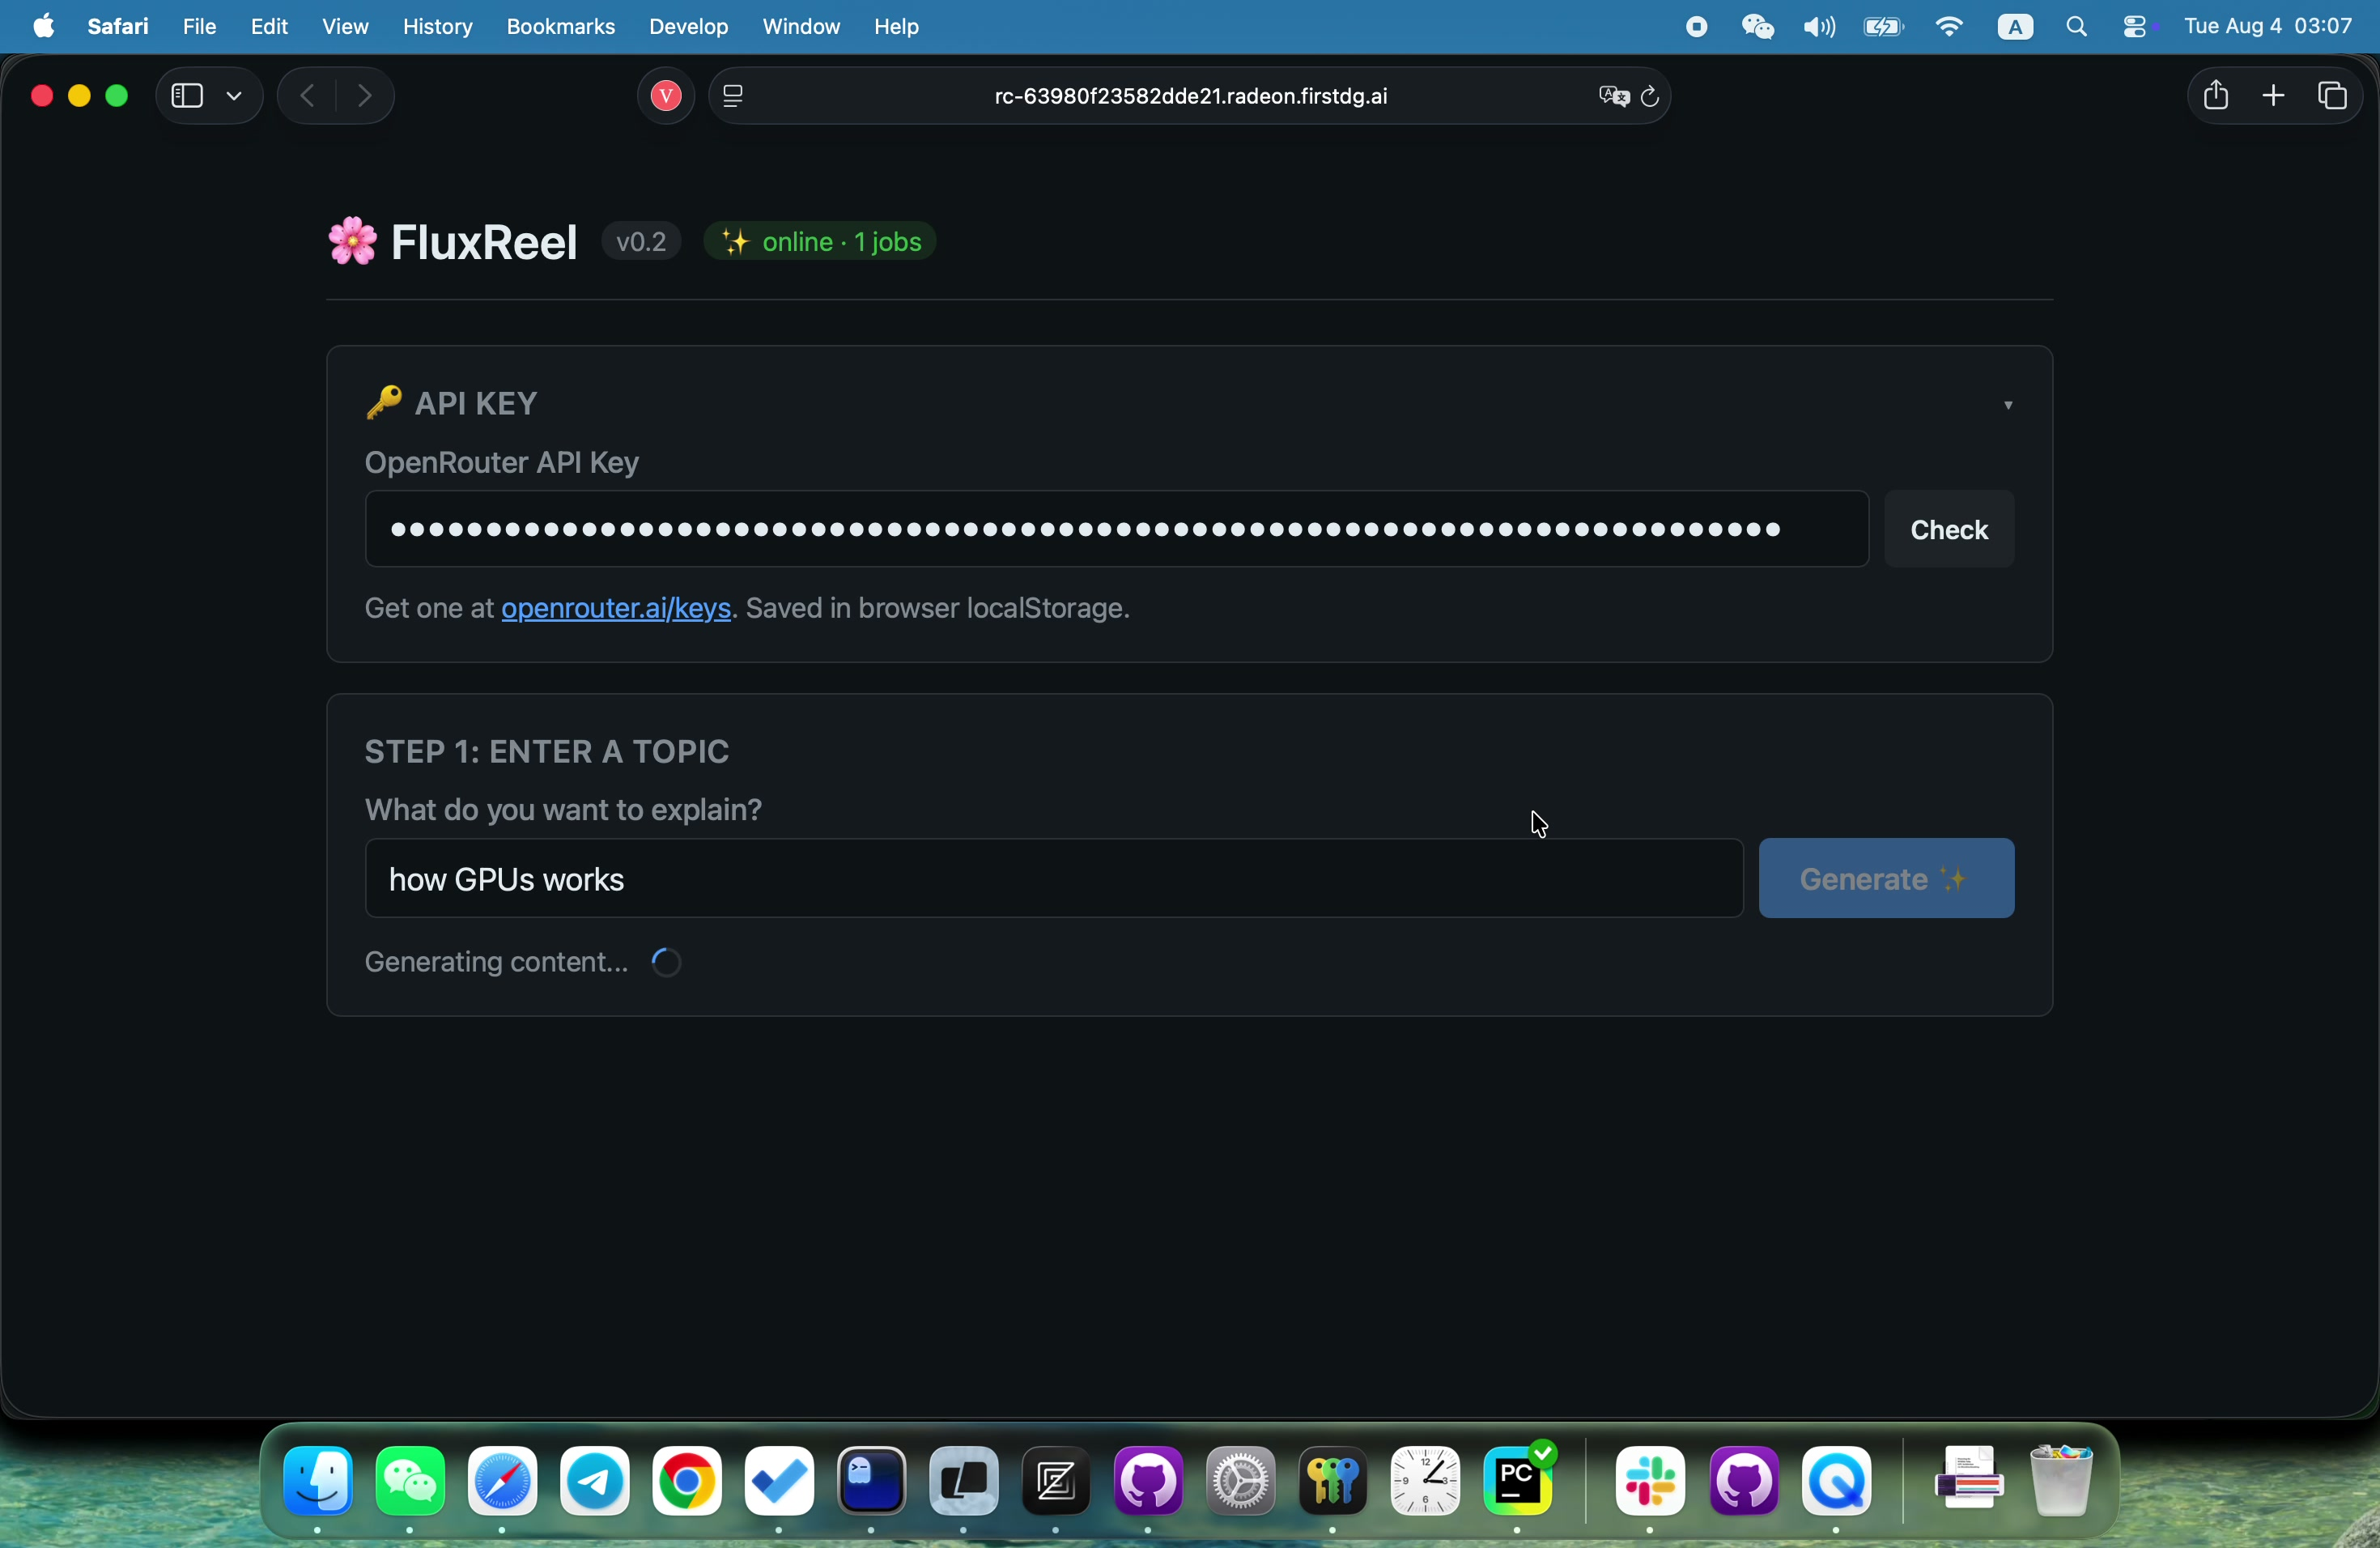
\includegraphics[width=\textwidth]{demo_frame_1.jpg}
  \caption{Sample video frame 1 --- scripted scene image composed with title bar.}
\end{figure}

\begin{figure}[htp]
  \centering
  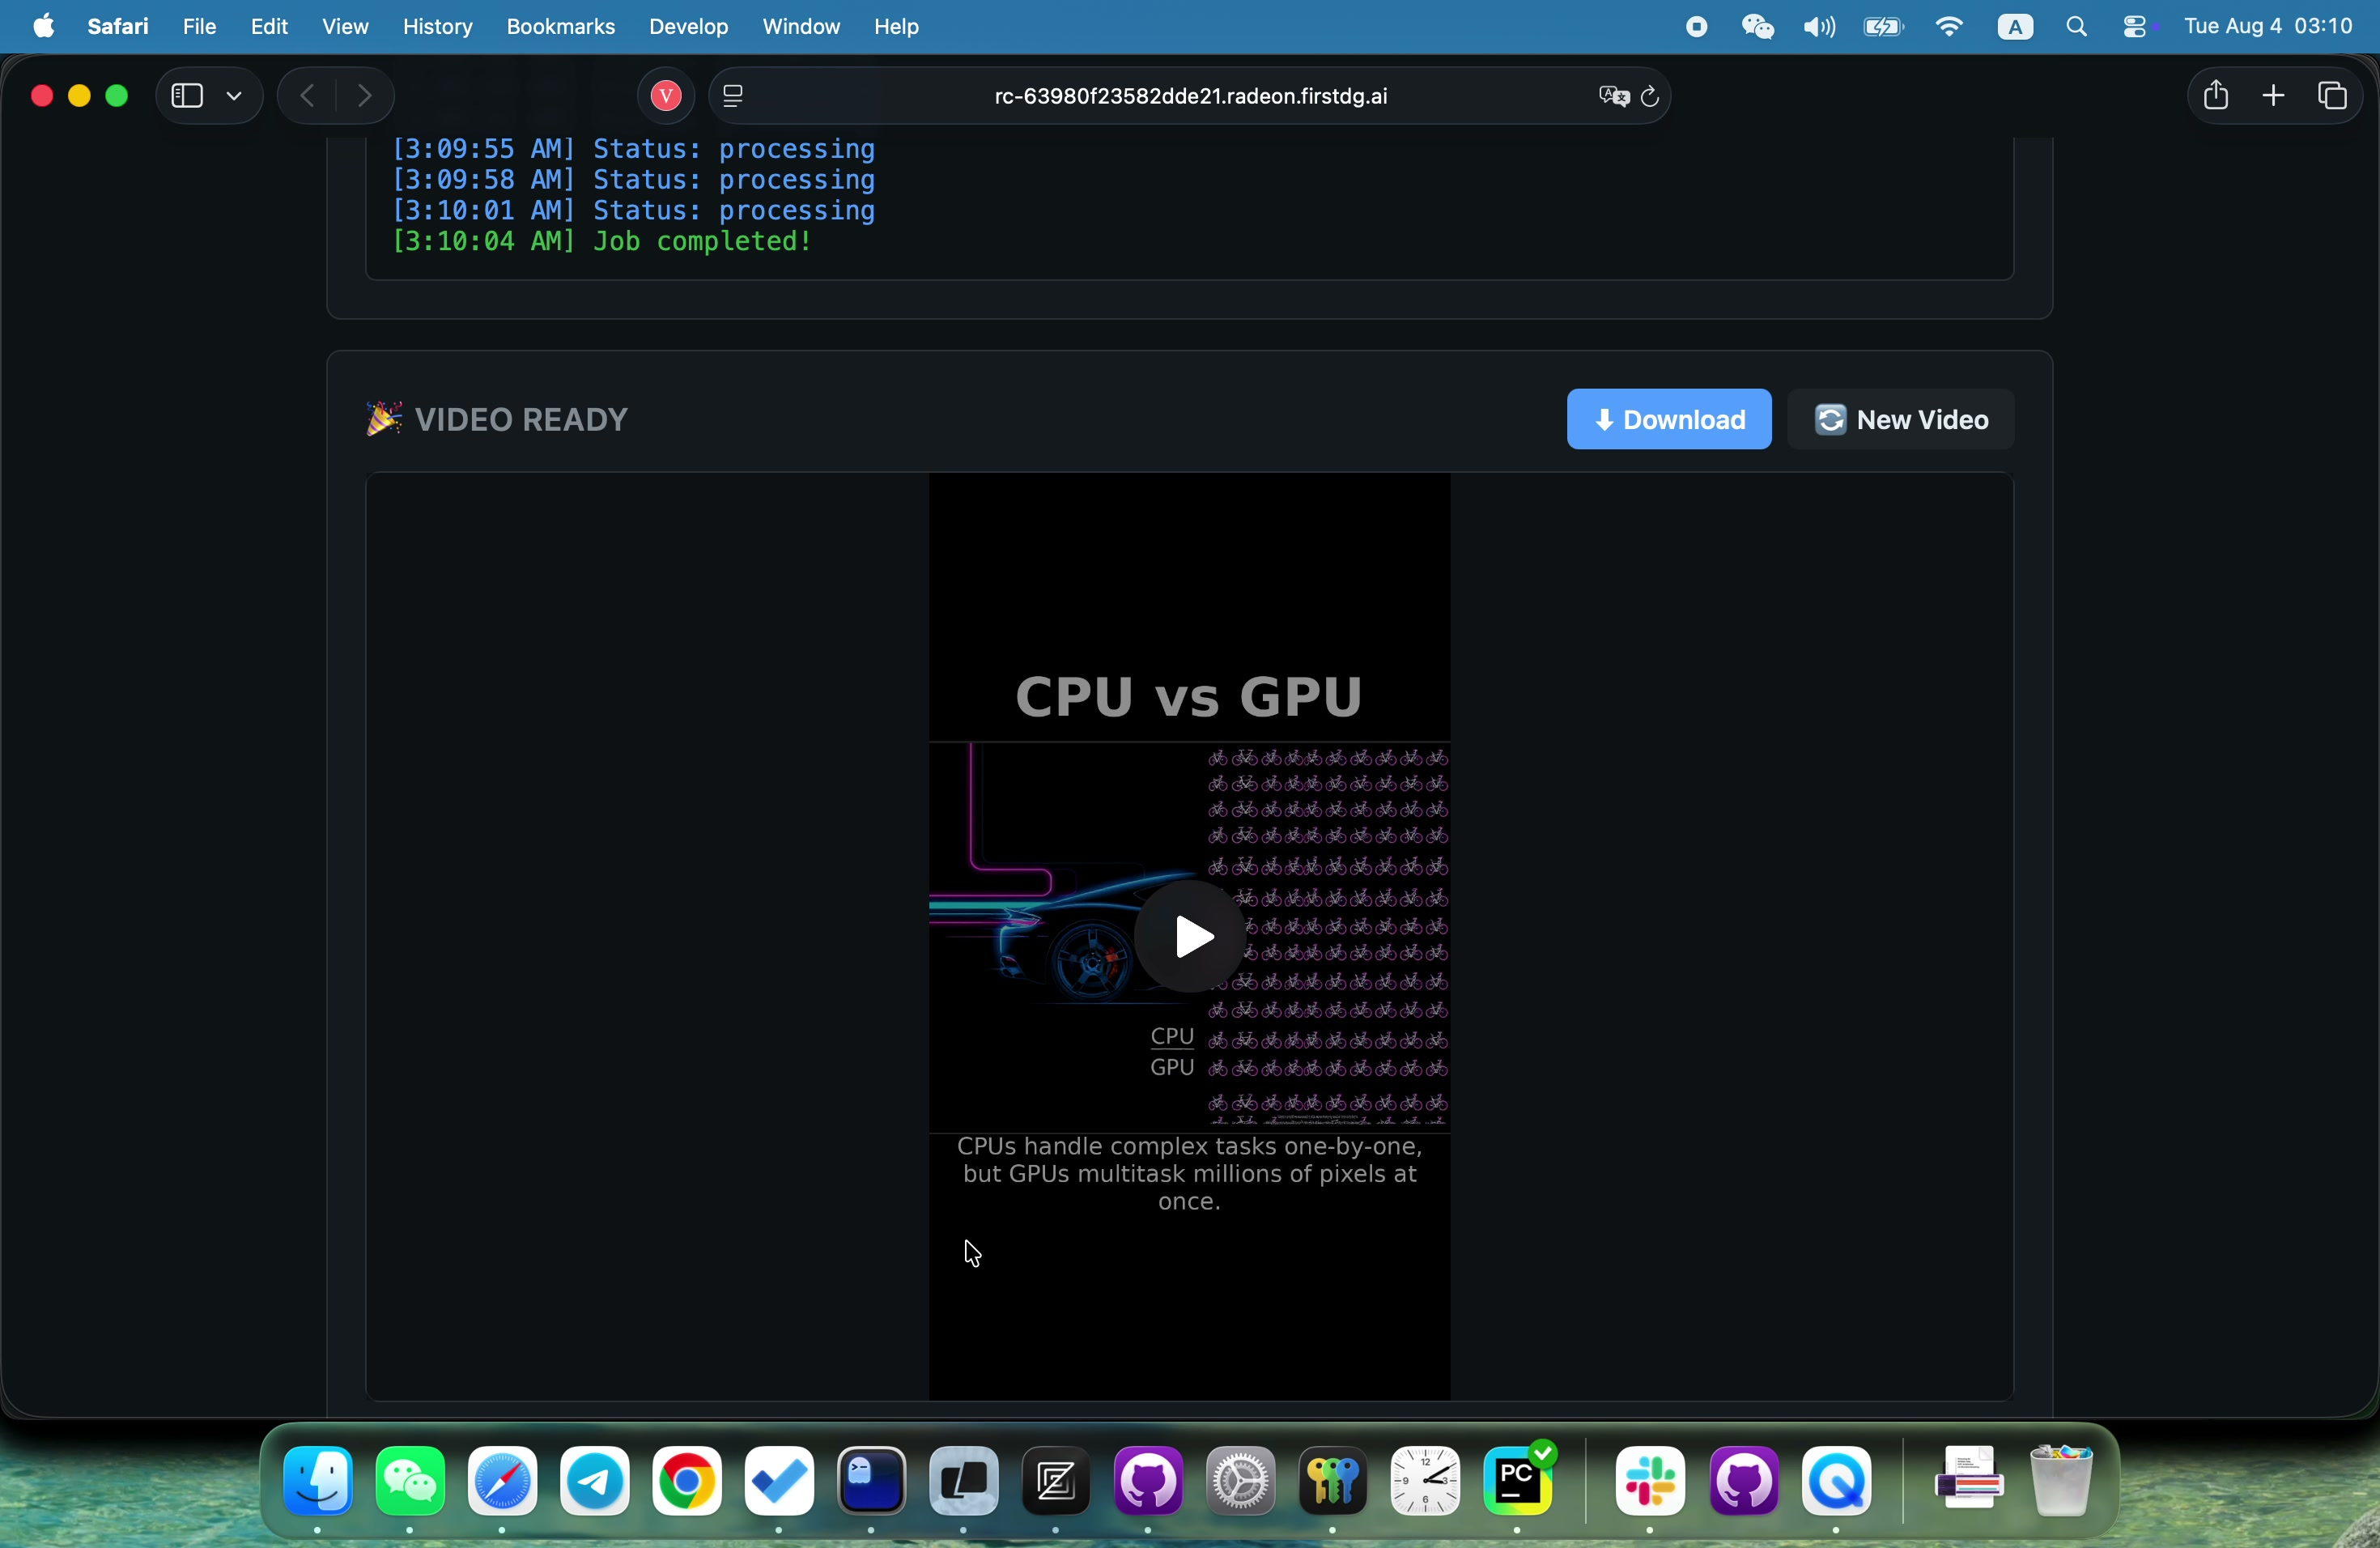
\includegraphics[width=\textwidth]{demo_frame_2.jpg}
  \caption{Sample video frame 2 --- scene image composed with subtitle bar.}
\end{figure}

\end{document}
